\section{Bases de datos relacionales. SQL}

En el modelo relacional las dos capas de diseño conceptual y lógico, se parecen mucho. Generalmente se implementan mediante \textbf{diagramas de Entidad/Relación} (modelo conceptual) y \textbf{tablas y relaciones} entre éstas (modelo lógico). Este es el modelo utilizado por los sistemas gestores de datos más habituales (SQL Server, Oracle, MySQL...) \cite{ref7}.

El modelo relacional de bases de datos se rige por algunas normas sencillas:

\begin{itemize}

\item Todos los datos se representan en forma de \textbf{tablas} (también llamadas “relaciones”, ver nota anterior). Incluso los resultados de consultar otras tablas. La tabla es además la unidad de almacenamiento principal.

\item Las tablas están compuestas por \textbf{filas} (o registros) y columnas (o campos) que almacenan cada uno de los registros (la información sobre una entidad concreta, considerados una unidad).

\item Las filas y las columnas, en principio, carecen de orden a la hora de ser almacenadas. Aunque en la implementación del diseño físico de cada SGBD esto no suele ser así. Por ejemplo, en SQL Server si añadimos una clave de tipo "Clustered" a una tabla haremos que los datos se ordenen físicamente por el campo correspondiente.

\item El orden de las columnas lo determina cada consulta (que se realizan usando SQL).

\item Cada tabla debe poseer una \textbf{clave primaria}, esto es, un \textbf{identificador único} de cada registro compuesto por una o más columnas

\item Para establecer una relación entre dos tablas es necesario incluir, en forma de columna, en una de ellas la clave primaria de la otra. A esta columna se le llama \textbf{clave externa}. Ambos conceptos de clave son extremadamente importantes en el diseño de bases de datos.

\end{itemize}

Sus principales ventajas son \cite{ref8} :

\begin{itemize}
\item \textbf{Mayor soporte y herramientas} debido a que lleva más tiempo en el mercado.

\item Es una tecnología ampliamente conocida y \textbf{los perfiles que lo conocen son mayoritarios} y más económicos.

\item Las bases de dato relacionales llevan una clase de “cabecera” que permite la \textbf{transaccionalidad entre tablas}. Esto significa que si hay un error durante la petición a cualquier nivel de la operación, se devuelve al punto inicial sin comprometer los datos que fueron utilizados durante el proceso.

\item Los datos deben cumplir con el tipo de dato definido en su estructura.
\end{itemize}

Sus principales inconvenientes son: 

\begin{itemize}
\item No es flexible; todos los objetos ingresados deben tener los mismos campos y estar correctamente validados.

\item El rendimiento y los recursos, mientras más compleja la base de datos y sus relaciones sea debido a la atomicidad, \textbf{necesita más procesamiento}.

\item La escalabilidad es reducida. Una aplicación con SQL \textbf{requiere un aumento de recursos de hardware} que generalmente son bastante costosos para escalar su rendimiento.
\end{itemize}

Algunas tecnologías SQL conocidas son:


\begin{figure}[H]
	\centering
	\begin{subfigure}[b]{0.25\textwidth}
		
\includegraphics[width=\textwidth,height=90px]{images/mysql}
		\caption{MySQL}
		\label{fig:mysql}
	\end{subfigure}
	~ 
	\begin{subfigure}[b]{0.25\textwidth}
		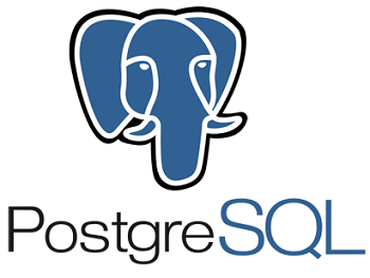
\includegraphics[width=\textwidth,height=90px]{images/postgres}
		\caption{PostgreSQL}
		\label{fig:postgresql}
	\end{subfigure}
	~ 
	\begin{subfigure}[b]{0.25\textwidth}
		
\includegraphics[width=\textwidth,height=90px]{images/sqlite}
		\caption{SQLite}
		\label{fig:sqlite}
	\end{subfigure}
	
	\begin{subfigure}[b]{0.25\textwidth}
		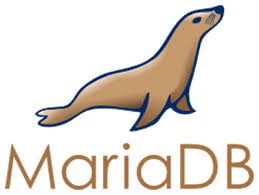
\includegraphics[width=\textwidth,height=90px]{images/mariadb}
		\caption{MariaDB}
		\label{fig:mariadb}
	\end{subfigure}
	~ 
	\begin{subfigure}[b]{0.25\textwidth}
		
\includegraphics[width=\textwidth,height=90px]{images/oracle}
		\caption{Oracle}
		\label{fig:oracle}
	\end{subfigure}
	~ 
	\begin{subfigure}[b]{0.25\textwidth}
		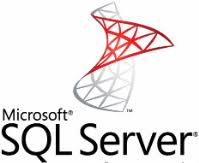
\includegraphics[width=\textwidth,height=90px]{images/sql_server}
		\caption{SQL-Server}
		\label{fig:sqlserver}
	\end{subfigure}
\end{figure}